% Options for packages loaded elsewhere
\PassOptionsToPackage{unicode}{hyperref}
\PassOptionsToPackage{hyphens}{url}
%
\documentclass[
]{book}
\usepackage{amsmath,amssymb}
\usepackage{lmodern}
\usepackage{iftex}
\ifPDFTeX
  \usepackage[T1]{fontenc}
  \usepackage[utf8]{inputenc}
  \usepackage{textcomp} % provide euro and other symbols
\else % if luatex or xetex
  \usepackage{unicode-math}
  \defaultfontfeatures{Scale=MatchLowercase}
  \defaultfontfeatures[\rmfamily]{Ligatures=TeX,Scale=1}
\fi
% Use upquote if available, for straight quotes in verbatim environments
\IfFileExists{upquote.sty}{\usepackage{upquote}}{}
\IfFileExists{microtype.sty}{% use microtype if available
  \usepackage[]{microtype}
  \UseMicrotypeSet[protrusion]{basicmath} % disable protrusion for tt fonts
}{}
\makeatletter
\@ifundefined{KOMAClassName}{% if non-KOMA class
  \IfFileExists{parskip.sty}{%
    \usepackage{parskip}
  }{% else
    \setlength{\parindent}{0pt}
    \setlength{\parskip}{6pt plus 2pt minus 1pt}}
}{% if KOMA class
  \KOMAoptions{parskip=half}}
\makeatother
\usepackage{xcolor}
\IfFileExists{xurl.sty}{\usepackage{xurl}}{} % add URL line breaks if available
\IfFileExists{bookmark.sty}{\usepackage{bookmark}}{\usepackage{hyperref}}
\hypersetup{
  pdftitle={Foraging: introducing our gaze-contingent eye-tracking paradigm for studying foraging},
  pdfauthor={Matthew Green},
  hidelinks,
  pdfcreator={LaTeX via pandoc}}
\urlstyle{same} % disable monospaced font for URLs
\usepackage{color}
\usepackage{fancyvrb}
\newcommand{\VerbBar}{|}
\newcommand{\VERB}{\Verb[commandchars=\\\{\}]}
\DefineVerbatimEnvironment{Highlighting}{Verbatim}{commandchars=\\\{\}}
% Add ',fontsize=\small' for more characters per line
\usepackage{framed}
\definecolor{shadecolor}{RGB}{248,248,248}
\newenvironment{Shaded}{\begin{snugshade}}{\end{snugshade}}
\newcommand{\AlertTok}[1]{\textcolor[rgb]{0.94,0.16,0.16}{#1}}
\newcommand{\AnnotationTok}[1]{\textcolor[rgb]{0.56,0.35,0.01}{\textbf{\textit{#1}}}}
\newcommand{\AttributeTok}[1]{\textcolor[rgb]{0.77,0.63,0.00}{#1}}
\newcommand{\BaseNTok}[1]{\textcolor[rgb]{0.00,0.00,0.81}{#1}}
\newcommand{\BuiltInTok}[1]{#1}
\newcommand{\CharTok}[1]{\textcolor[rgb]{0.31,0.60,0.02}{#1}}
\newcommand{\CommentTok}[1]{\textcolor[rgb]{0.56,0.35,0.01}{\textit{#1}}}
\newcommand{\CommentVarTok}[1]{\textcolor[rgb]{0.56,0.35,0.01}{\textbf{\textit{#1}}}}
\newcommand{\ConstantTok}[1]{\textcolor[rgb]{0.00,0.00,0.00}{#1}}
\newcommand{\ControlFlowTok}[1]{\textcolor[rgb]{0.13,0.29,0.53}{\textbf{#1}}}
\newcommand{\DataTypeTok}[1]{\textcolor[rgb]{0.13,0.29,0.53}{#1}}
\newcommand{\DecValTok}[1]{\textcolor[rgb]{0.00,0.00,0.81}{#1}}
\newcommand{\DocumentationTok}[1]{\textcolor[rgb]{0.56,0.35,0.01}{\textbf{\textit{#1}}}}
\newcommand{\ErrorTok}[1]{\textcolor[rgb]{0.64,0.00,0.00}{\textbf{#1}}}
\newcommand{\ExtensionTok}[1]{#1}
\newcommand{\FloatTok}[1]{\textcolor[rgb]{0.00,0.00,0.81}{#1}}
\newcommand{\FunctionTok}[1]{\textcolor[rgb]{0.00,0.00,0.00}{#1}}
\newcommand{\ImportTok}[1]{#1}
\newcommand{\InformationTok}[1]{\textcolor[rgb]{0.56,0.35,0.01}{\textbf{\textit{#1}}}}
\newcommand{\KeywordTok}[1]{\textcolor[rgb]{0.13,0.29,0.53}{\textbf{#1}}}
\newcommand{\NormalTok}[1]{#1}
\newcommand{\OperatorTok}[1]{\textcolor[rgb]{0.81,0.36,0.00}{\textbf{#1}}}
\newcommand{\OtherTok}[1]{\textcolor[rgb]{0.56,0.35,0.01}{#1}}
\newcommand{\PreprocessorTok}[1]{\textcolor[rgb]{0.56,0.35,0.01}{\textit{#1}}}
\newcommand{\RegionMarkerTok}[1]{#1}
\newcommand{\SpecialCharTok}[1]{\textcolor[rgb]{0.00,0.00,0.00}{#1}}
\newcommand{\SpecialStringTok}[1]{\textcolor[rgb]{0.31,0.60,0.02}{#1}}
\newcommand{\StringTok}[1]{\textcolor[rgb]{0.31,0.60,0.02}{#1}}
\newcommand{\VariableTok}[1]{\textcolor[rgb]{0.00,0.00,0.00}{#1}}
\newcommand{\VerbatimStringTok}[1]{\textcolor[rgb]{0.31,0.60,0.02}{#1}}
\newcommand{\WarningTok}[1]{\textcolor[rgb]{0.56,0.35,0.01}{\textbf{\textit{#1}}}}
\usepackage{longtable,booktabs,array}
\usepackage{calc} % for calculating minipage widths
% Correct order of tables after \paragraph or \subparagraph
\usepackage{etoolbox}
\makeatletter
\patchcmd\longtable{\par}{\if@noskipsec\mbox{}\fi\par}{}{}
\makeatother
% Allow footnotes in longtable head/foot
\IfFileExists{footnotehyper.sty}{\usepackage{footnotehyper}}{\usepackage{footnote}}
\makesavenoteenv{longtable}
\usepackage{graphicx}
\makeatletter
\def\maxwidth{\ifdim\Gin@nat@width>\linewidth\linewidth\else\Gin@nat@width\fi}
\def\maxheight{\ifdim\Gin@nat@height>\textheight\textheight\else\Gin@nat@height\fi}
\makeatother
% Scale images if necessary, so that they will not overflow the page
% margins by default, and it is still possible to overwrite the defaults
% using explicit options in \includegraphics[width, height, ...]{}
\setkeys{Gin}{width=\maxwidth,height=\maxheight,keepaspectratio}
% Set default figure placement to htbp
\makeatletter
\def\fps@figure{htbp}
\makeatother
\setlength{\emergencystretch}{3em} % prevent overfull lines
\providecommand{\tightlist}{%
  \setlength{\itemsep}{0pt}\setlength{\parskip}{0pt}}
\setcounter{secnumdepth}{5}
\usepackage{booktabs}
\ifLuaTeX
  \usepackage{selnolig}  % disable illegal ligatures
\fi
\usepackage[]{natbib}
\bibliographystyle{apalike}

\title{Foraging: introducing our gaze-contingent eye-tracking paradigm for studying foraging}
\author{Matthew Green}
\date{Thursday 12 May 2022 at 11:12:06}

\begin{document}
\maketitle

{
\setcounter{tocdepth}{1}
\tableofcontents
}
\hypertarget{first-things-first}{%
\chapter{First things first}\label{first-things-first}}

Things about the series of two experiments before we consider experiment one and experiment two separately.

\hypertarget{part-experiment-one}{%
\part{Experiment One}\label{part-experiment-one}}

\hypertarget{introduction}{%
\chapter{Introduction}\label{introduction}}

In experiment 1, the computerized gaze contingent task consisted of 20 individual trials. In each trial participants were presented with a display containing 30 trees, 15 of which contained a hidden fruit item which was the target (the target was an apple, represented by a filled red circle). On each trial, the participant's task was to forage for and retrieve 10 of the 15 fruit items.

We manipulated one factor within-subjects (Resource Distribution) with 2 levels: `clumped' and `random'.

We created ten random stimuli in which the 15 target fruit items were uniformly distributed about the 30 trees (random condition) and ten stimuli in which all 15 target fruit items were arranged in one large patch (clumped condition) that covered either the left or the right side of the layout.

This line runs the code that gets the individual participant results files in.

\begin{Shaded}
\begin{Highlighting}[]
\CommentTok{\# source("e1\_process\_individual\_results\_files.R", local = knitr::knit\_global())}
\end{Highlighting}
\end{Shaded}

\hypertarget{number-of-trees}{%
\chapter{Number of Trees}\label{number-of-trees}}

Contents

\hypertarget{trial-duration}{%
\chapter{Trial Duration}\label{trial-duration}}

Contents

\hypertarget{revisits-per-trial}{%
\chapter{Revisits Per Trial}\label{revisits-per-trial}}

Experiment 1

\hypertarget{raw-data}{%
\section{Raw data}\label{raw-data}}

This line reads in the dataset that results from collating the results files for each participant.

\begin{Shaded}
\begin{Highlighting}[]
\NormalTok{e1 }\OtherTok{\textless{}{-}} \FunctionTok{readRDS}\NormalTok{(}\StringTok{"fgms\_e1\_allsubs.rds"}\NormalTok{)}
\end{Highlighting}
\end{Shaded}

This renames the raw data but doesn't do any operations on it.

\begin{Shaded}
\begin{Highlighting}[]
\CommentTok{\# this tibble is one row for each tree visited saying whether it was a revisit or not}
\NormalTok{e1\_revisits }\OtherTok{\textless{}{-}}
\NormalTok{  e1 }\SpecialCharTok{\%\textgreater{}\%}
  \FunctionTok{transmute}\NormalTok{(}
    \AttributeTok{pp           =}\NormalTok{ pid,}
    \AttributeTok{condition    =}\NormalTok{ R,}
    \AttributeTok{stage        =} \FunctionTok{as\_factor}\NormalTok{(}\FunctionTok{ifelse}\NormalTok{(trial}\SpecialCharTok{\textless{}=}\DecValTok{5}\NormalTok{, }\StringTok{"early"}\NormalTok{, }\StringTok{"late"}\NormalTok{)),}
    \AttributeTok{progress     =} \FunctionTok{as\_factor}\NormalTok{(trial),}
    \AttributeTok{index        =}\NormalTok{ index,}
    \AttributeTok{tree         =}\NormalTok{ tile,}
    \AttributeTok{is\_a\_revisit =}\NormalTok{ revisit}
\NormalTok{  )}
\end{Highlighting}
\end{Shaded}

\hypertarget{aggregation-1-trial-counts}{%
\section{Aggregation 1: Trial counts}\label{aggregation-1-trial-counts}}

\begin{Shaded}
\begin{Highlighting}[]
\CommentTok{\# First level of aggregation collapses over index and yields }
\CommentTok{\# a count for each trial: }
\CommentTok{\# each row is how many revisits they made on that trial}
\CommentTok{\# THESE ARE TRIAL SUMS}
\NormalTok{TRIAL\_SUMS }\OtherTok{\textless{}{-}}
\NormalTok{  e1\_revisits }\SpecialCharTok{\%\textgreater{}\%} 
  \FunctionTok{group\_by}\NormalTok{(pp, condition, stage, progress) }\SpecialCharTok{\%\textgreater{}\%} 
  \FunctionTok{summarise}\NormalTok{(}\AttributeTok{nrevisits =} \FunctionTok{sum}\NormalTok{(is\_a\_revisit), }\AttributeTok{.groups =} \StringTok{"drop\_last"}\NormalTok{)}
\end{Highlighting}
\end{Shaded}

\hypertarget{aggregation-2-participant-means}{%
\section{Aggregation 2: Participant means}\label{aggregation-2-participant-means}}

\begin{Shaded}
\begin{Highlighting}[]
\CommentTok{\# Second level of aggregation collapses over trials}
\CommentTok{\# each row is the average number of revisits that participant }
\CommentTok{\# made in that combination of random/clumped and early/late}
\CommentTok{\# THESE ARE PARTICIPANT MEANS}
\NormalTok{PARTICIPANT\_MEANS }\OtherTok{\textless{}{-}} 
\NormalTok{  TRIAL\_SUMS }\SpecialCharTok{\%\textgreater{}\%} 
  \FunctionTok{group\_by}\NormalTok{(pp, condition, stage) }\SpecialCharTok{\%\textgreater{}\%} 
  \FunctionTok{summarise}\NormalTok{(}\AttributeTok{meanrevisits=}\FunctionTok{mean}\NormalTok{(nrevisits), }\AttributeTok{.groups=}\StringTok{"drop\_last"}\NormalTok{)}
\end{Highlighting}
\end{Shaded}

\hypertarget{descriptives}{%
\section{Descriptives}\label{descriptives}}

Condition descriptives

\begin{Shaded}
\begin{Highlighting}[]
\CommentTok{\# To generate mean and sd properly for each level of condition }
\CommentTok{\# (clumped/random), we first need data with one clumped score }
\CommentTok{\# for each participant and one random score for each }
\CommentTok{\# participant, averaging over early and late stages.}
\NormalTok{tempCond }\OtherTok{\textless{}{-}}\NormalTok{ PARTICIPANT\_MEANS }\SpecialCharTok{\%\textgreater{}\%} 
  \FunctionTok{group\_by}\NormalTok{(pp,condition) }\SpecialCharTok{\%\textgreater{}\%} \FunctionTok{summarise}\NormalTok{(}\AttributeTok{cmeans=}\FunctionTok{mean}\NormalTok{(meanrevisits))}
\CommentTok{\# Now we can ask for means and sd for clumped and random }
\CommentTok{\# that each pp contributed one value to}
\NormalTok{CONDITION\_DESCRIPTIVES }\OtherTok{\textless{}{-}}\NormalTok{ tempCond }\SpecialCharTok{\%\textgreater{}\%} 
  \FunctionTok{group\_by}\NormalTok{(condition) }\SpecialCharTok{\%\textgreater{}\%} 
  \FunctionTok{summarise}\NormalTok{(}\AttributeTok{mean=}\FunctionTok{mean}\NormalTok{(cmeans), }\AttributeTok{sd=}\FunctionTok{sd}\NormalTok{(cmeans))}
\CommentTok{\# issue the table}
\NormalTok{CONDITION\_DESCRIPTIVES }\SpecialCharTok{\%\textgreater{}\%} 
  \FunctionTok{gt}\NormalTok{() }\SpecialCharTok{\%\textgreater{}\%} 
  \FunctionTok{tab\_header}\NormalTok{(}\StringTok{"Revisits per trial descriptives"}\NormalTok{) }\SpecialCharTok{\%\textgreater{}\%} 
  \FunctionTok{fmt\_number}\NormalTok{(}\AttributeTok{columns =} \FunctionTok{c}\NormalTok{(}\StringTok{"mean"}\NormalTok{,}\StringTok{"sd"}\NormalTok{), }\AttributeTok{decimals=}\DecValTok{2}\NormalTok{) }\SpecialCharTok{\%\textgreater{}\%} 
  \FunctionTok{gtsave}\NormalTok{(}\StringTok{"e1\_tables/condition\_means.png"}\NormalTok{)}
\end{Highlighting}
\end{Shaded}

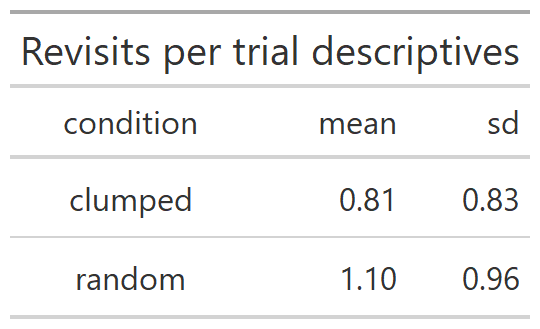
\includegraphics[width=0.33\linewidth]{e1_figures/CONDITION_DESCRIPTIVES-1}

Stage descriptives

\begin{Shaded}
\begin{Highlighting}[]
\CommentTok{\# To generate mean and sd properly for each level of stage,}
\CommentTok{\# we first need to collapse over condition (clumped/random)}
\CommentTok{\# to get one score for each participant per level of stage}
\CommentTok{\# (early/late)}
\NormalTok{tempStage }\OtherTok{\textless{}{-}}\NormalTok{ PARTICIPANT\_MEANS }\SpecialCharTok{\%\textgreater{}\%} 
  \FunctionTok{group\_by}\NormalTok{(pp,stage) }\SpecialCharTok{\%\textgreater{}\%} 
  \FunctionTok{summarise}\NormalTok{(}\AttributeTok{smeans=}\FunctionTok{mean}\NormalTok{(meanrevisits))}
\CommentTok{\# Now we can ask for means and sd per level of stage}
\NormalTok{STAGE\_DESCRIPTIVES }\OtherTok{\textless{}{-}}\NormalTok{ tempStage  }\SpecialCharTok{\%\textgreater{}\%} 
  \FunctionTok{group\_by}\NormalTok{(stage) }\SpecialCharTok{\%\textgreater{}\%} 
  \FunctionTok{summarise}\NormalTok{(}\AttributeTok{mean=}\FunctionTok{mean}\NormalTok{(smeans),}\AttributeTok{sd=}\FunctionTok{sd}\NormalTok{(smeans))}
\CommentTok{\# issue the table}
\NormalTok{STAGE\_DESCRIPTIVES }\SpecialCharTok{\%\textgreater{}\%} 
  \FunctionTok{gt}\NormalTok{() }\SpecialCharTok{\%\textgreater{}\%} 
  \FunctionTok{tab\_header}\NormalTok{(}\StringTok{"Revisits per trial descriptives"}\NormalTok{) }\SpecialCharTok{\%\textgreater{}\%} 
  \FunctionTok{fmt\_number}\NormalTok{(}\AttributeTok{columns =} \FunctionTok{c}\NormalTok{(}\StringTok{"mean"}\NormalTok{,}\StringTok{"sd"}\NormalTok{), }\AttributeTok{decimals=}\DecValTok{2}\NormalTok{) }\SpecialCharTok{\%\textgreater{}\%} 
  \FunctionTok{gtsave}\NormalTok{(}\StringTok{"e1\_tables/stage\_means.png"}\NormalTok{)}
\end{Highlighting}
\end{Shaded}

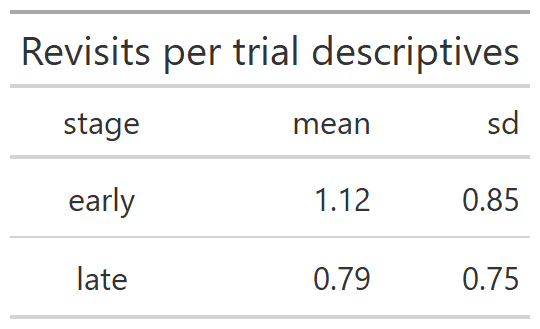
\includegraphics[width=0.33\linewidth]{e1_figures/STAGE_DESCRIPTIVES-1}

SxC Descriptives

\begin{Shaded}
\begin{Highlighting}[]
\CommentTok{\# To get the 2 x 2 interaction means, yielding a 2x2 table with mean and sd}
\NormalTok{SxC\_DESCRIPTIVES }\OtherTok{\textless{}{-}}\NormalTok{ PARTICIPANT\_MEANS }\SpecialCharTok{\%\textgreater{}\%} \FunctionTok{group\_by}\NormalTok{(condition,stage) }\SpecialCharTok{\%\textgreater{}\%} \FunctionTok{summarise}\NormalTok{(}\AttributeTok{mean=}\FunctionTok{mean}\NormalTok{(meanrevisits),}\AttributeTok{sd=}\FunctionTok{sd}\NormalTok{(meanrevisits))}
\NormalTok{SxC\_DESCRIPTIVES }\SpecialCharTok{\%\textgreater{}\%} 
  \FunctionTok{gt}\NormalTok{(}\AttributeTok{rowname\_col =} \StringTok{"stage"}\NormalTok{, }\AttributeTok{groupname\_col =} \StringTok{"condition"}\NormalTok{) }\SpecialCharTok{\%\textgreater{}\%} 
  \FunctionTok{tab\_stubhead}\NormalTok{(}\AttributeTok{label =} \StringTok{"condition"}\NormalTok{) }\SpecialCharTok{\%\textgreater{}\%} 
  \FunctionTok{fmt\_number}\NormalTok{(}\AttributeTok{columns =} \FunctionTok{c}\NormalTok{(}\StringTok{"mean"}\NormalTok{,}\StringTok{"sd"}\NormalTok{), }\AttributeTok{decimals=}\DecValTok{2}\NormalTok{) }\SpecialCharTok{\%\textgreater{}\%} 
  \FunctionTok{tab\_header}\NormalTok{(}\StringTok{"Revisits per trial descriptives"}\NormalTok{) }\SpecialCharTok{\%\textgreater{}\%} 
  \FunctionTok{gtsave}\NormalTok{(}\StringTok{"e1\_tables/SxC\_means.png"}\NormalTok{)}
\end{Highlighting}
\end{Shaded}

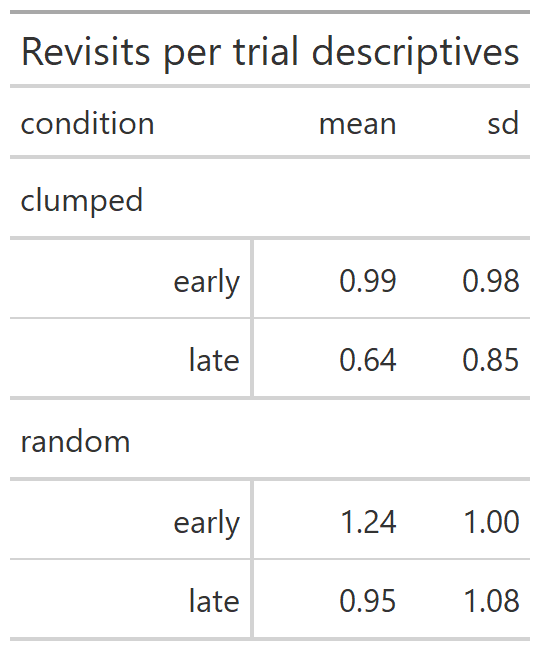
\includegraphics[width=0.33\linewidth]{e1_figures/SxC_Descriptives-1}

\hypertarget{plots}{%
\section{Plots}\label{plots}}

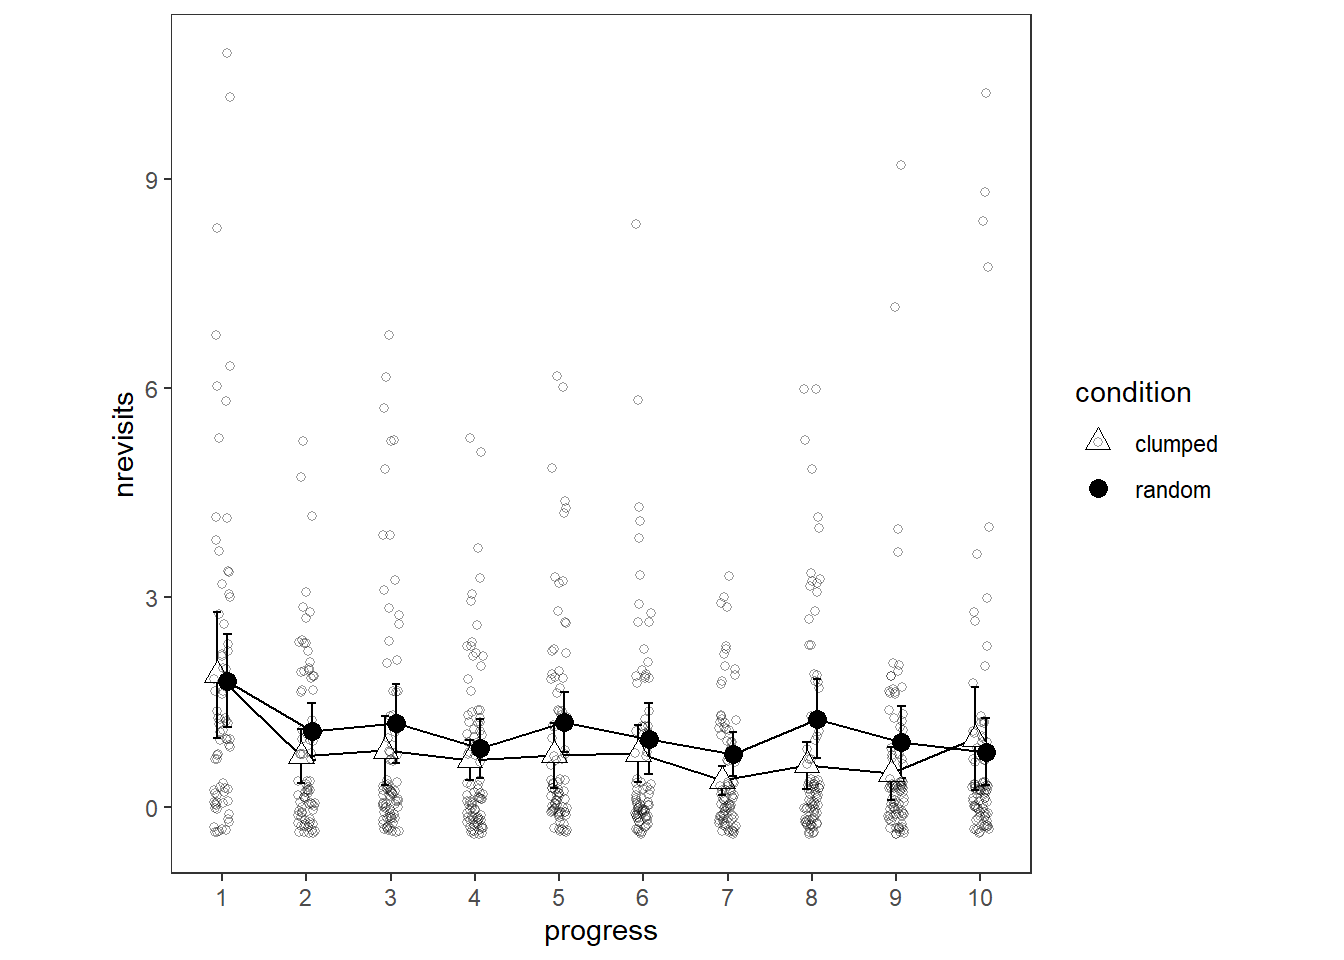
\includegraphics[width=0.5\linewidth]{e1_figures/progress-revisits-1}

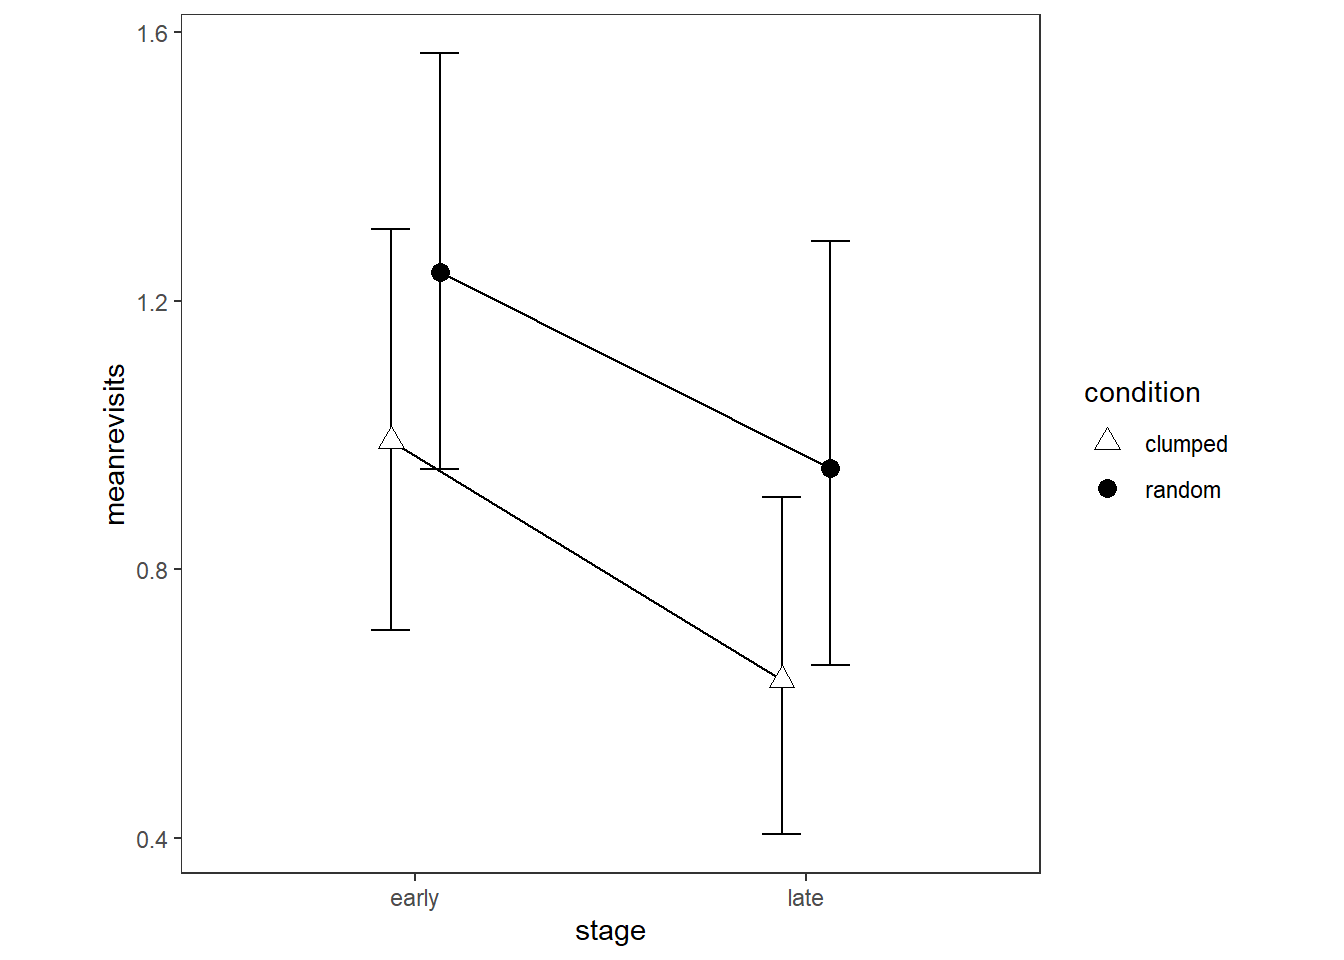
\includegraphics[width=0.5\linewidth]{e1_figures/stage-revisits-1}

\hypertarget{anova}{%
\section{ANOVA}\label{anova}}

\begin{Shaded}
\begin{Highlighting}[]
\NormalTok{ez1 }\OtherTok{\textless{}{-}} \FunctionTok{ezANOVA}\NormalTok{(}
  \AttributeTok{data=}\NormalTok{PARTICIPANT\_MEANS,}
  \AttributeTok{wid=}\NormalTok{pp,}
  \AttributeTok{within=}\FunctionTok{.c}\NormalTok{(condition, stage),}
  \AttributeTok{dv=}\NormalTok{meanrevisits}
\NormalTok{)}
\end{Highlighting}
\end{Shaded}

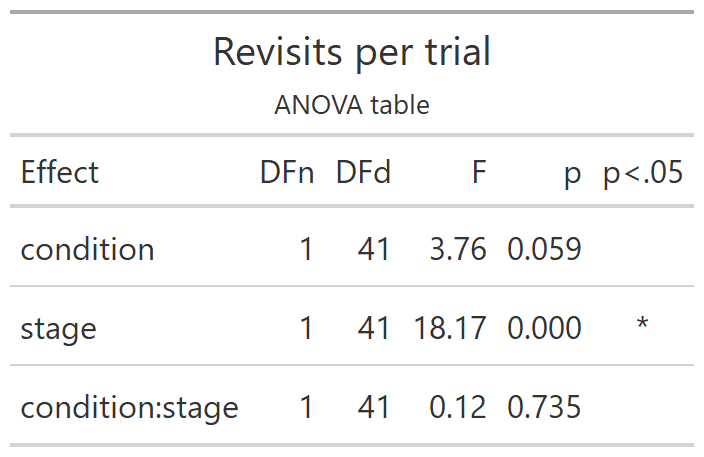
\includegraphics[width=0.33\linewidth]{e1_figures/anova-table-revisits-1}

\hypertarget{retrieval-rate}{%
\chapter{Retrieval Rate}\label{retrieval-rate}}

Contents

\hypertarget{inter-tree-distance}{%
\chapter{Inter-tree distance}\label{inter-tree-distance}}

Contents

\hypertarget{part-experiment-two}{%
\part{Experiment Two}\label{part-experiment-two}}

\hypertarget{introduction-1}{%
\chapter{Introduction}\label{introduction-1}}

Contents

In experiment 2, n trials. Task.

We manipulated two factors: one within-subjects (Resource Distribution) with two levels: `clumped' and `random'; and one between-subjects (Fading) with two levels `fade' and `no-fade'. The fade condition differeed from experiment 1 in that once a tree had been visited, it was thereafter displayed faded out such that it was apparent to the participant which trees had been visited previously and which had not. The no-fade condition was the same as experiment 1. We expected that the fading would function as a memory aid and reduce revisits as well as making the task easier overall on the other metrics.

We created ?? random stimuli in which the ?? target fruit items were uniformly distributed about the ?? trees (random condition) and ?? stimuli in which all ?? target fruit items were arranged in one large area (clumped condition) that covered either the left or the right side of the layout.

This line runs the code that gets the individual participant results files in.

\begin{Shaded}
\begin{Highlighting}[]
\FunctionTok{source}\NormalTok{(}\StringTok{"e2\_process\_individual\_results\_files.R"}\NormalTok{, }\AttributeTok{local =}\NormalTok{ knitr}\SpecialCharTok{::}\FunctionTok{knit\_global}\NormalTok{())}
\CommentTok{\#\textgreater{} }
\CommentTok{\#\textgreater{}  *********************************************************** }
\CommentTok{\#\textgreater{}           Loading standardize package version 0.2.2          }
\CommentTok{\#\textgreater{}      Call standardize.news() to see new features/changes     }
\CommentTok{\#\textgreater{}  ***********************************************************}
\CommentTok{\#\textgreater{} {-}{-} Attaching packages {-}{-}{-}{-}{-}{-}{-}{-}{-}{-}{-}{-}{-}{-}{-}{-}{-}{-}{-} tidyverse 1.3.1 {-}{-}}
\CommentTok{\#\textgreater{} v ggplot2 3.3.6     v purrr   0.3.4}
\CommentTok{\#\textgreater{} v tibble  3.1.7     v dplyr   1.0.9}
\CommentTok{\#\textgreater{} v tidyr   1.2.0     v stringr 1.4.0}
\CommentTok{\#\textgreater{} v readr   2.1.2     v forcats 0.5.1}
\CommentTok{\#\textgreater{} {-}{-} Conflicts {-}{-}{-}{-}{-}{-}{-}{-}{-}{-}{-}{-}{-}{-}{-}{-}{-}{-}{-}{-}{-}{-} tidyverse\_conflicts() {-}{-}}
\CommentTok{\#\textgreater{} x dplyr::filter() masks stats::filter()}
\CommentTok{\#\textgreater{} x dplyr::lag()    masks stats::lag()}
\CommentTok{\#\textgreater{} P001 done}
\CommentTok{\#\textgreater{} P002 done}
\CommentTok{\#\textgreater{} P003 done}
\CommentTok{\#\textgreater{} P004 done}
\CommentTok{\#\textgreater{} P005 done}
\CommentTok{\#\textgreater{} P006 done}
\CommentTok{\#\textgreater{} P007 done}
\CommentTok{\#\textgreater{} P008 done}
\CommentTok{\#\textgreater{} P009 done}
\CommentTok{\#\textgreater{} P010 done}
\CommentTok{\#\textgreater{} P011 done}
\CommentTok{\#\textgreater{} P012 done}
\CommentTok{\#\textgreater{} P013 done}
\CommentTok{\#\textgreater{} P014 done}
\CommentTok{\#\textgreater{} P015 done}
\CommentTok{\#\textgreater{} P016 done}
\CommentTok{\#\textgreater{} P017 done}
\CommentTok{\#\textgreater{} P018 done}
\CommentTok{\#\textgreater{} P019 done}
\CommentTok{\#\textgreater{} P020 done}
\CommentTok{\#\textgreater{} P021 done}
\CommentTok{\#\textgreater{} P022 done}
\CommentTok{\#\textgreater{} P023 done}
\CommentTok{\#\textgreater{} P024 done}
\CommentTok{\#\textgreater{} P025 done}
\CommentTok{\#\textgreater{} P026 done}
\CommentTok{\#\textgreater{} P027 done}
\CommentTok{\#\textgreater{} P028 done}
\CommentTok{\#\textgreater{} P029 done}
\CommentTok{\#\textgreater{} P030 done}
\CommentTok{\#\textgreater{} P031 done}
\CommentTok{\#\textgreater{} P032 done}
\CommentTok{\#\textgreater{} P033 done}
\CommentTok{\#\textgreater{} P034 done}
\CommentTok{\#\textgreater{} P035 done}
\CommentTok{\#\textgreater{} P036 done}
\CommentTok{\#\textgreater{} P037 done}
\CommentTok{\#\textgreater{} P038 done}
\CommentTok{\#\textgreater{} P039 done}
\CommentTok{\#\textgreater{} P040 done}
\CommentTok{\#\textgreater{} P041 done}
\CommentTok{\#\textgreater{} P042 done}
\end{Highlighting}
\end{Shaded}

\hypertarget{number-of-trees-1}{%
\chapter{Number of trees}\label{number-of-trees-1}}

Experiment 2

Load the libraries.

This line reads in the dataset that results from collating the results files for each participant.

\begin{Shaded}
\begin{Highlighting}[]
\NormalTok{e2 }\OtherTok{\textless{}{-}} \FunctionTok{readRDS}\NormalTok{(}\StringTok{"fgms\_e2\_allsubs.rds"}\NormalTok{)}
\end{Highlighting}
\end{Shaded}

This renames the raw data but doesn't do any operations on it.

\begin{Shaded}
\begin{Highlighting}[]
\CommentTok{\# this tibble is one row for each tree visited saying whether it was a revisit or not}
\NormalTok{e2\_revisits }\OtherTok{\textless{}{-}}
\NormalTok{  e2 }\SpecialCharTok{\%\textgreater{}\%}
  \FunctionTok{transmute}\NormalTok{(}
    \AttributeTok{pp           =}\NormalTok{ participant,}
    \AttributeTok{trial        =}\NormalTok{ trial\_number,}
    \AttributeTok{resources    =} \FunctionTok{factor}\NormalTok{(R, }\AttributeTok{levels=}\FunctionTok{c}\NormalTok{(}\StringTok{".pat"}\NormalTok{,}\StringTok{"dis"}\NormalTok{), }\AttributeTok{labels=}\FunctionTok{c}\NormalTok{(}\StringTok{"clumped"}\NormalTok{, }\StringTok{"random"}\NormalTok{)),}
    \AttributeTok{stage        =} \FunctionTok{as\_factor}\NormalTok{(}\FunctionTok{ifelse}\NormalTok{(trial}\SpecialCharTok{\textless{}=}\DecValTok{10}\NormalTok{, }\StringTok{"early"}\NormalTok{, }\StringTok{"late"}\NormalTok{)),}
    \AttributeTok{progress     =} \FunctionTok{factor}\NormalTok{(trial),}
    \AttributeTok{index        =}\NormalTok{ index,}
    \AttributeTok{tree         =}\NormalTok{ tile,}
    \AttributeTok{is\_a\_revisit =}\NormalTok{ revisit}
\NormalTok{  )}
\end{Highlighting}
\end{Shaded}

Here

\hypertarget{trial-duration-1}{%
\chapter{Trial Duration}\label{trial-duration-1}}

E2

\hypertarget{revisits-per-trial-1}{%
\chapter{Revisits Per Trial}\label{revisits-per-trial-1}}

Experiment 2

\hypertarget{raw-data-1}{%
\section{Raw data}\label{raw-data-1}}

This line reads in the dataset that results from collating the results files for each participant.

\begin{Shaded}
\begin{Highlighting}[]
\NormalTok{e2 }\OtherTok{\textless{}{-}} \FunctionTok{readRDS}\NormalTok{(}\StringTok{"fgms\_e2\_allsubs.rds"}\NormalTok{)}
\end{Highlighting}
\end{Shaded}

\hypertarget{retrieval-rate-1}{%
\chapter{Retrieval Rate}\label{retrieval-rate-1}}

E2

\hypertarget{inter-tree-distance-1}{%
\chapter{Inter-tree-distance}\label{inter-tree-distance-1}}

E2

\hypertarget{appendix-appendices}{%
\appendix}


\hypertarget{appendix-a}{%
\chapter{Appendix A}\label{appendix-a}}

Content \ldots{}

\hypertarget{appendix-b}{%
\chapter{Appendix B}\label{appendix-b}}

Content \ldots{}

  \bibliography{book.bib,packages.bib}

\end{document}
